\chapter{Eksperyment LHCb}

Niniejszy rozdział stanowi krótkie wprowadzenie do eksperymentu LHCb (ang. Large Hadron Collider beauty expermient).

\section{Akcelerator LHC}
\indent LHC jest największym, działającym akceleratorem cząstek na świecie zaprojektowanym do zderzania protonów przy energii środka masy $\sqrt{s}=14 TeV$. Poza samą energia wiązki ważnym parametrem związanym z~ pracą akceleratora jest  świetlność ($L$). Wielkość, ta mówi jak wiele zaszło zderzeń na sekundę oraz jest związana z przekrojem czynnym:
\begin{equation}
\frac{dN}{dt} =L \sigma
\end{equation}
Łączny rozmiar zebranych danych można otrzymać całkując chwilową świetlność:
\begin{equation}
\mathcal{L} = \int L dt
\end{equation}
Otrzymana wielkość posiada jednostkę odwrotności pola powierzchni, zwaną również barnem. Eksperymenty ATLAS oraz CMS (opisane poniżej) mogą pracować z maksymalną osiągalną świetlnością przez LHC-$\mathcal{L}=10^{34}cm^{-2}s^{-1}$, natomiast LHCb dla swoich potrzeb redukuje ją w celu zmniejszenia  wielokrotnych zderzeń dla pojedynczego zderzenia. 

LHC został umiejscowiony w 26,7 km tunelu skonstruowanym pierwotnie dla poprzedniego akceleratora elektronowego LEP (ang. Large Electron–Positron Collider). 
\begin{figure}[h]
  \centering
  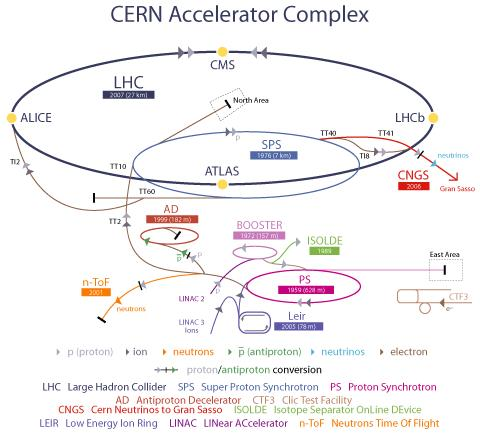
\includegraphics[scale=1.1]{rozdzial2/AccComple.jpeg}
  % AccComple.gif: 480x434 pixel, 72dpi, 16.93x15.31 cm, bb=0 0 480 434
  \caption{Schemat kompleksu przyspieszającego akceleratora LHC. \cite{public}}
  \label{fig:AccComplex}
\end{figure}

Na rysunku \ref{fig:AccComplex} pokazany jest schemat kompleksu przyspieszającego oraz detektorów pracujących przy eksperymencie LHC. Sam proces przyspieszania jest wielostopniowy\cite{Haefeli}.
Na początku protony otrzymywane są w wyniku jonizacji atomów wodoru po czym wstępnie przyspieszane w akceleratorze liniowym (LINIAC2) do energii 500MeV. Następnie dwa kołowe akceleratory zwiększają energie cząstek do 1GeV (BOOSTER) oraz 26 GeV (PS), kontynuując podróż przez system akceleratorów  przechodzą przez SPS rozpędzający je do energii 450 GeV. Na sam koniec są umieszczane w docelowym pierścieniu LHC. W którym to przebywają 20 minut zanim nabiorą maksymalną energię. Do utrzymania dwóch przeciwbieżnych wiązek protonowych na ich orbitach potrzebne są 1232 nadprzewodzące magnesy, generujące pole o indukcji 8.33T. Aby magnesy pozostawały w stanie nadprzewodzenia muszą być schłodzone do temperatury 1.9 K. Tak niską temperaturę uzyskuje się przy użyciu nadciekłego helu. 

Wiązki są zderzane w 4 punktach oznaczonych na rysunku \ref{fig:AccComplex} żółtymi kropkami. W każdym z tych punktów umiejscowiony jest jeden z detektorów oraz powiązanych z nimi eksperyment. Noszą one odpowiednio nazwy ATLAS, CMS, ALICE oraz LHCb.

Głównymi celami eksperymentów ATLAS (ang. A Toroidal Lhc ApparatuS)\cite{ATLAS} oraz CMS (ang. Compact Muon Solenoid) \cite{CMS} jest poszukiwanie bozonu Higgsa, cząstki która wg Modelu Standardowego odpowiada za nadawanie masy, oraz sprawdzenie teorii supersymetrii (SUSY). ALICE (ang. A Large Ion Collider Experiment)\cite{ALICE} został zoptymalizowany do badania plazmy gluonowo-kwarkowej powstającej w wyniku zderzeń ciężkich jonów.


\section{Detektor LHCb}
Eksperyment LHCb został zaprojektowany do badania łamania symetrii kombinowanej \textbf{CP} oraz rzadkich procesów w sektorze ciężkich kwarków $b$ i $c$. Jako przykład można podać mezon B. Produkcja pary $b\overline{b}$ będąca wynikiem zderzenia proton-proton jest zdominowana przez fuzje gluonową  gluonów i partonów, diagram Feynmana opisujący takie procesy został umieszczony na rysunku \ref{fig:feynman}.

 Amplituda takiego procesu jest proporcjonalna do kwadratu stałej oddziaływań silnych. Warto zwrócić uwagę, że w przeciwieństwie do oddziaływań elektromagnetycznych, dla których stała sprzężenie jest równa:
 \begin{equation}
 \alpha_{QED}=\frac{e^2}{4\pi \hbar c}\approx \frac{1}{137} 
 \end{equation}
Stałe sprzężenia oddziaływań silnych zmieniają się z odległościami pomiędzy kwarkami \cite{perkins}. Symulacje takich procesów pokazały, że przy energiach osiąganych dzięki LHC, zarazem kwarki b jak i  $\overline{b}$ przeważnie produkowane są w kierunku do przodu lub tyłu, co przedstawiono na rysunku\ref{fig:pythia}.  


\begin{figure}[h]
  \centering
  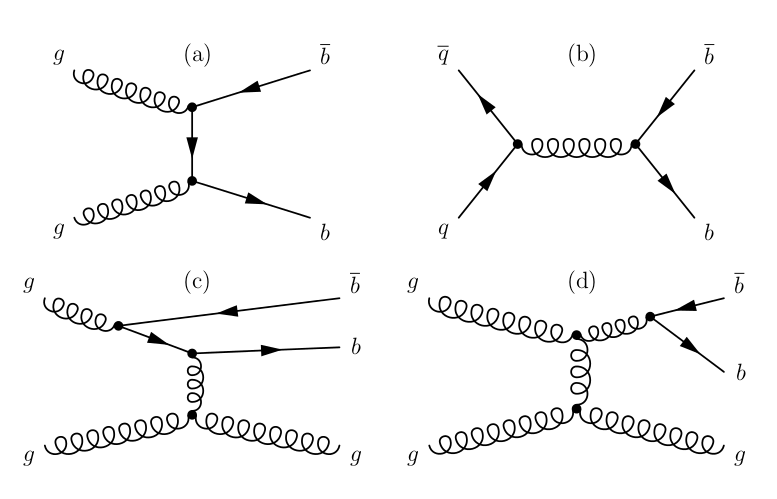
\includegraphics[scale=0.5]{rozdzial2/Feynman.png}
  % AccComple.gif: 480x434 pixel, 72dpi, 16.93x15.31 cm, bb=0 0 480 434
  \caption{Przykładowe diagramy Feynmana obrazujące produkcję mezonów B. Diagramy pierwszego rzędu odpowiadają kreacji par przez fuzję gluonową (a) oraz anihilację kwark-antykwark(b). Przykładowe schematy wyższych rzędów to wzbudzenia zapachowe (c) oraz rozszczepianie gluonu(d)}
  \label{fig:feynman}
\end{figure}



\begin{figure}[h]
  \centering
  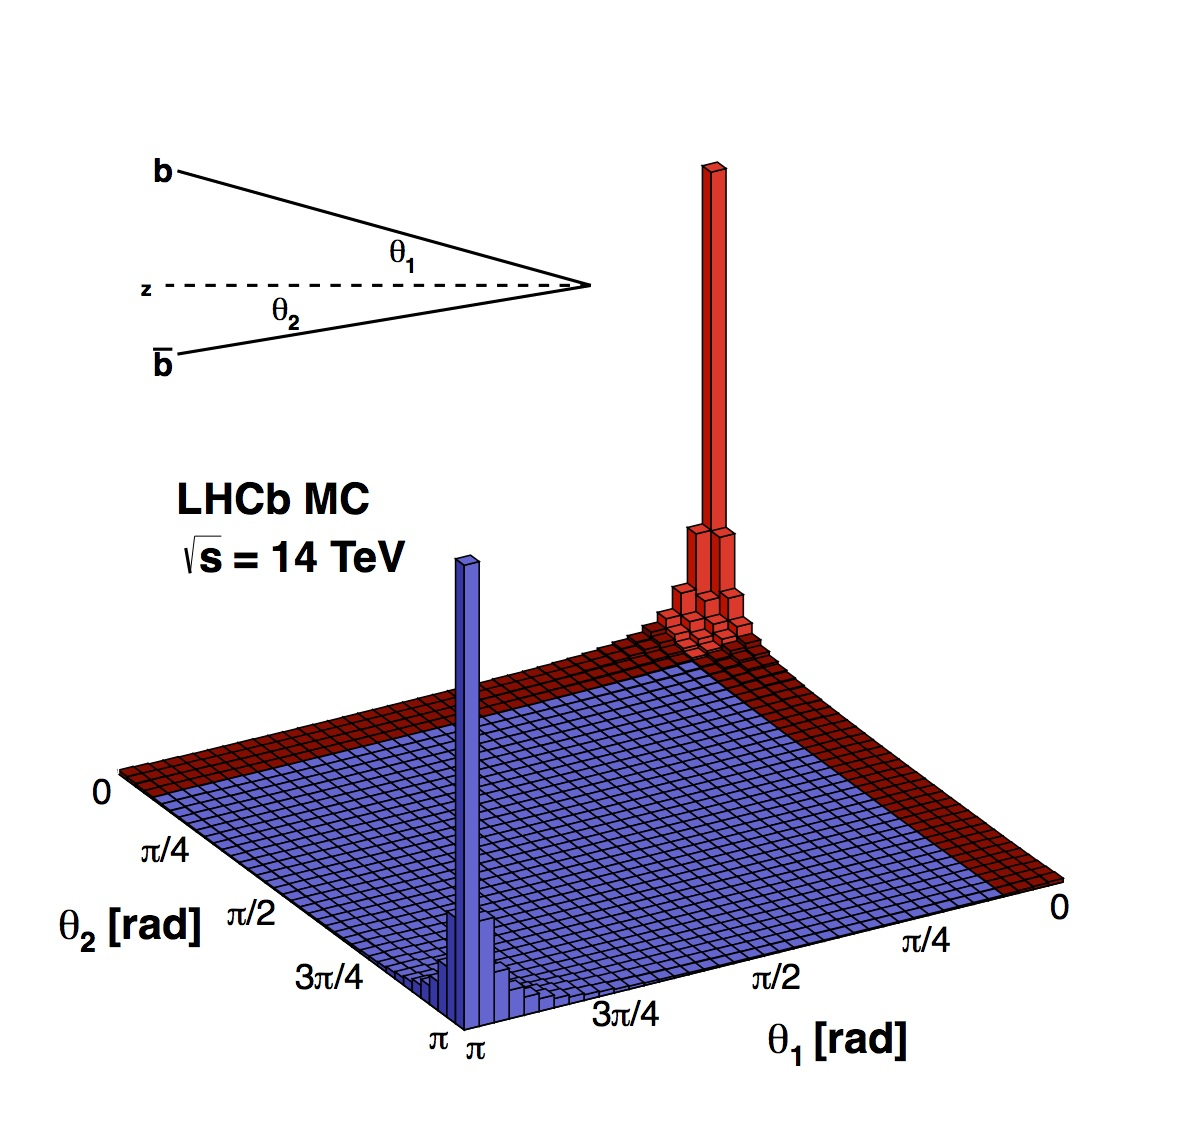
\includegraphics[scale=0.7]{rozdzial2/pythia.jpg}
  % AccComple.gif: 480x434 pixel, 72dpi, 16.93x15.31 cm, bb=0 0 480 434
  \caption{Wykres korelacji pomiędzy kątem polarnym a ilością produkowanych kwarków b w zderzeniu proton-proton. Symulacja została wykonana przy użyciu programu Pythia \cite{public}}
  \label{fig:pythia}
\end{figure}

Detektor LHCb jest spektrometrem o akceptanci kątowej wynoszącej od 10 do 300 mrad. Jest to geometria typu "do przodu", której konsekwencją jest efektywny przedział pseudorapidity obserwowanych cząstek $1.7<\eta < 5.3$ . Przy czym pseudorapidity, $\eta $ jest zdefiniowana jako
\begin{equation}
 \eta=-\ln\left(\tan\frac{\theta}{2}\right)
\end{equation}
gdzie $\theta$ kąt między kierunkiem pędu cząstki oraz osią wiązki.


\begin{figure}[h]  \centering
  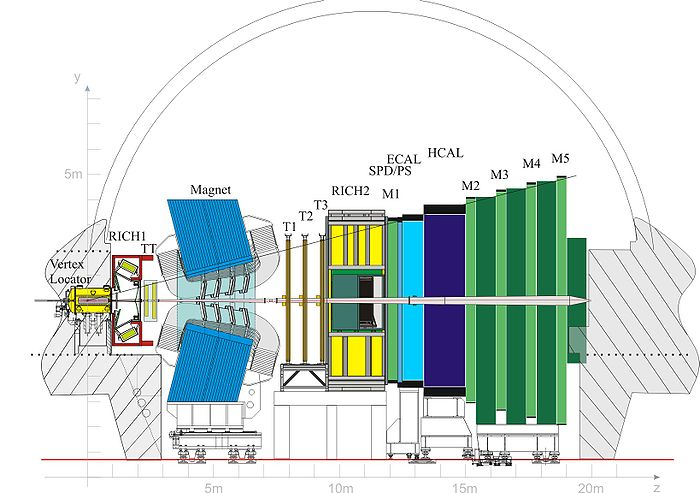
\includegraphics[scale=0.6]{rozdzial2/Lhcbview.jpg}
  % Lhcbview.jpg: 700x493 pixel, 150dpi, 11.85x8.35 cm, bb=0 0 336 237
  \caption{Detektor LHCb w całej okazałości \cite{public}}
  \label{fig:Layout}
\end{figure}

Zamieszczony na rysunku \ref{fig:Layout} spektrometr LHCb składa się z szeregu systemów detekcyjnych. Systemy te są podzielone na trzy główne grupy. Pierwsza z nich służy do  rekonstrukcji śladów cząstek naładowanych. Informacja o śladach niezbędna jest do wyznaczania trzech komponentów pędu i położenia cząstek. Następna grupa detektorów odpowiedzialna jest za identyfikację cząstek. Te dwie informacje w pełni opisują każdą indywidualną cząstkę, a co za tym idzie całe zdarzenie. Ostatecznie układ wyzwalania (ang. trigger) dokonuje selekcji przypadków na te, ciekawe z punktu widzenia analizy fizycznej. 
\begin{itemize}
\item \textbf{Rekonstrukcja śladów}: System rekonstrukcji śladów składa się z położonego najbliżej punktu zderzeń, mikropaskowego, krzemowego detektora zwanego VELO (ang. VErtex LOcator) który, z  bardzo dużą precyzją,   mierzy pozycję pierwotnego wierzchołka oraz parametr zderzenia (ang. Impact Parameter). Wizualizacja parametru zderzenia znajduje się na rysunku \ref{fig:IP}.
\begin{figure}[th] 
  \centering
  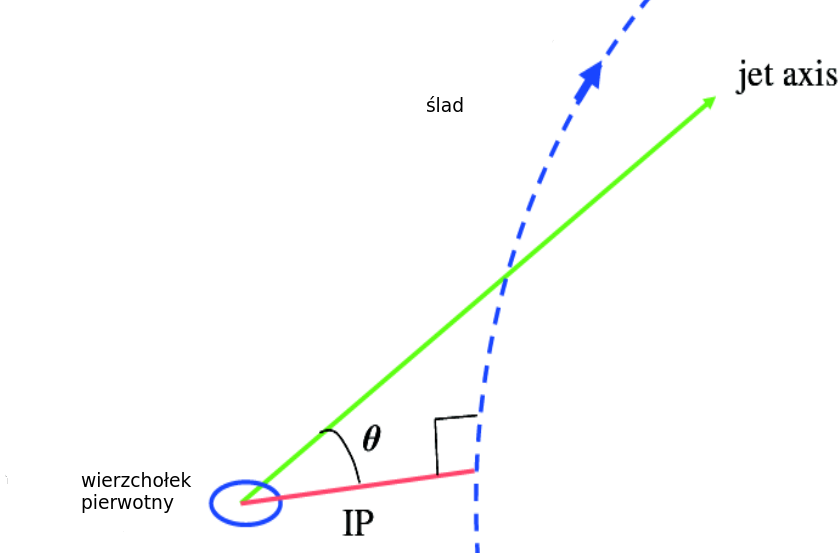
\includegraphics[scale=0.5]{rozdzial2/impactParameter.png}
  \caption{Wizualizacja parametru zderzenia, będącego najmniejszą odległością od wierzchołka pierwotnego do śladu. Parametr zderzenia został oznaczony czerwoną linią. }
  \label{fig:IP}
\end{figure}

Następnym, po detektorze VELO, jest umiejscowiony przed magnesem zakrzywiającym detektor TT (ang. Tracker Turicensis). Podobnie jak wcześniej wspomniany VELO, TT również został wykonany w technologii mikropaskowej. Zadaniem jego jest zwiększenie rozdzielczości mierzonego pędu cząstek. Pole magnetyczne wytwarzane przez magnes dipolowy zakrzywia trajektorię ruchu cząstek w płaszczyźnie x-z, co umożliwia wyznaczanie ich pędu poprzez porównywanie elementów toru przed oraz za magnesem. System śladowy jest dopełniany przez stacje T, które to wraz z VELO, pozwalają wyznaczać pęd oraz kierunek ruchu cząstek. Stacje T dzielą się na dwa regiony. Pierwszy, znajdujący się bliżej rury akceleratora, składa się z~ mikroposkowych detektorów krzemowych, natomiast ten bardziej oddalony jest  gazowym detektorem słomkowym.
Każdy z detektorów do wyznaczania śladów charakteryzuje się wystarczająca rozdzielczością przestrzenną. 

\item \textbf{Identyfikacja cząstek}: Zasada działania systemu identyfikacji cząstek jest oparta na dwóch prawach fizycznych. Pierwszym z nich jest emisja promieniowania Czerenkowa. Promieniowanie to jest emitowane gdy naładowana cząstka porusza się w danym ośrodku szybciej niż światło w tym ośrodku. Kąt emitowanego fotonu jest zależny od prędkości z jaką porusza się cząstka wg wzoru
\begin{equation}
 cos\theta=\frac{c}{n v}
\end{equation}
gdzie:\\
c- prędkość światłą w próżni, v- prędkość cząstki, n- współczynnik załamania ośrodka. Jak pokazano na rysunku \ref{fig:RICH} 

 Zjawisko to wykorzystują  dwa detektory RICH (ang. Ring Imaging Cherenkov detector). Efekt ten pozwala na rozróżnienie pomiędzy typami hadronów. 

Elektromagnetyczne oraz hadronowe kalorymetry, ECAL i HCAL, mierzą energię oddziałujących z nimi cząstek poprzez całkowitą ich absorpcję. Detektory te wspierane są przez SPD oraz PS, które to pomagają w rozwiązywaniu występujących dwuznaczności w identyfikacji. Ostatnim elementem czynnym, w znaczeniu oddalenia od miejsca  zajścia zderzenia, w systemie detekcyjnym LHCb jest układ detektorów mionowych. Układ ten, jak sama nazwa wskazuje, jest wykorzystywany do identyfikacji mionów. Jego stacje (od M1 do M5) rejestrują cząstki, które przemierzyły całą długość detektora LHCb. Tylko miony, z naładowanych cząstek, posiadają takie własności. 
\end{itemize} 
Komponenty wchodzące w skład detektora są dokładnie opisane w dalszej części tego rozdziału. 

\subsection{Magnes zakrzywiający}
Jednym z istotnych elementów systemu rekonstrukcji śladów cząstek naładowanych jest magnes dipolowy, który zakrzywia trajektorie cząstek, co daje możliwość pomiaru pędu. Składa się z dwóch identycznych, aluminiowych, jednocześnie nie będących w stanie nadprzewodnictwa cewek umiejscowionych symetrycznie w około osi wiązki.

Magnes ten wytwarza pole o maksymalnej indukcji o wartości $B_{max}=1.1T$ oraz siłę gięcia równą $\int B dl=4Tm$ \cite{magnet}. W celu poprawy ewentualnych korelacji związanych z kierunkiem odchylania, możliwa jest zamiana polaryzacji magnesu. Diagram prezentujący wygląd magnesu został zamieszczony na rysunku \ref{fig:magnes}.
\begin{figure}[!ht]
 \centering
 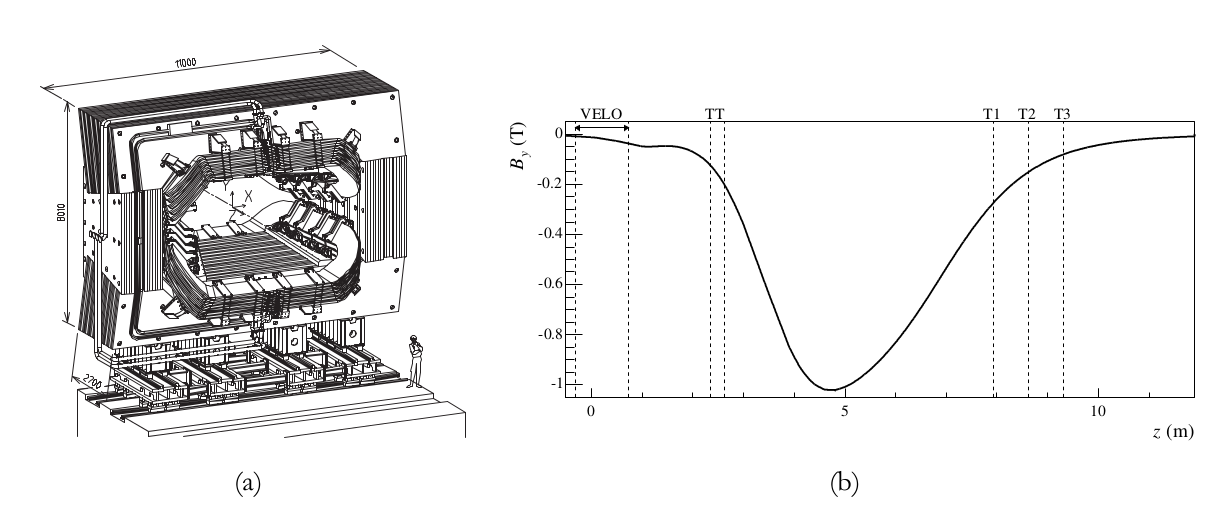
\includegraphics[scale=0.35]{rozdzial2/magnes.png}
 % Velo_jakis.png: 637x464 pixel, 96dpi, 16.85x12.28 cm, bb=0 0 478 348
 \caption{Schemat magnesu zakrzywiającego wchodzącego w skład systemu detekcyjnego LHCb(a) oraz wielkość składowej y-owej indukcji pola magnetycznego jako funkcja współrzędnej z-owej.  }
 \label{fig:magnes}
\end{figure}

 


\subsection{VELO}
\label{VELO}

VELO (ang. VErtex LOcator) to mikropaskowy detektor krzemowy specjalnie zaprojektowany do rekonstrukcji pierwotnego oraz wtórnych wierzchołków powstającego w wyniku rozpadu mezonu $B_{(s)}^0$ oraz $D_{(s)}^0$\cite{VELORaport}. Obszar detekcji znajduje się już 8 mm od osi wiązki. W celu kontroli skutków efektów radiacyjnych układ stale utrzymywany jest w obniżonej temperaturze \cite{Papadelis} . Pomiary dokonywane przez detektor są wykorzystywane również przez tryger wysokiego poziomu (HLT). 
\begin{figure}[!ht]
 \centering
 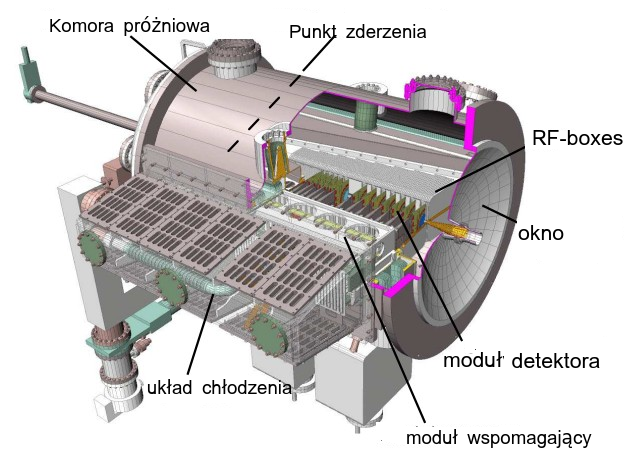
\includegraphics[scale=0.7]{rozdzial2/Velo_jakis.png}
 % Velo_jakis.png: 637x464 pixel, 96dpi, 16.85x12.28 cm, bb=0 0 478 348
 \caption{Schemat detektora VELO\cite{VELORaport}}
 \label{fig:SchematVELO}
\end{figure}
\subsubsection{Sensory krzemowe }
Pozycjo-czułe elementy VELO składają się z jednostronnych detektorów półprzewodnikowych o grubości 300$\mu m$ i  kształcie zaprezentowanym na rysunku \ref{fig:sensory}, akceptacja kątowa wynosi $182^{o}$, przy czym $2^{o}$ jest to obszar pokryty przez dwa przeciwległe sensory. Wyróżniamy dwa typy sensorów. Jedne, służące do pomiaru współrzędnej radialnej R, drugie mierzą składową azymutalną $\Phi$. Każdy sensor zawiera 2048 fizycznych kanałów pomiarowych. 
\begin{figure}[ht!]
 \centering
 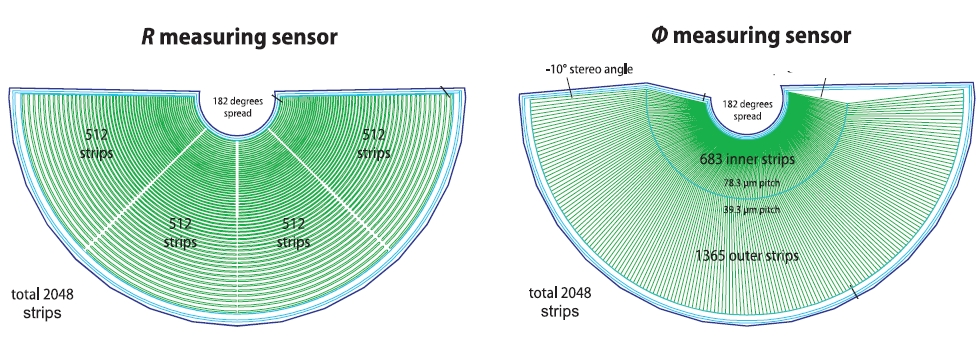
\includegraphics[scale=0.6]{rozdzial2/sensory.jpeg}
 % sensory.jpeg: 622x384 pixel, 96dpi, 16.46x10.16 cm, bb=0 0 467 288
 \caption{Geometria sensorów \cite{VELORaport}}
 \label{fig:sensory}
\end{figure}

Na \ref{fig:sensory} przedstawiona jest różnica w geometrii pasków. Paski w sensorach typu R są wycinkami współśrodkowych okręgów. Paski, te podzielone są na 4 segmenty . Natomiast sensory $\Phi$ dzielą się radialnie na dwie części- zewnętrzną (638 pasków) oraz wewnętrzną(1365 pasków), przy czym paski w każdej z części posiadają kąty "stereo" o przeciwnych znakach.
\subsubsection{Elektronika odczytu}
Beetle reprezentuje typ układów elektroniki front-end. Jest to ASIC (ang.  Application Specific Integrated Circuit) czyli dedykowany układ scalony mający za zadanie odczyt oraz kształtowanie impulsów zarejestrowanych przez sensory VELO.  Na \ref{fig:Beetle_Block} został przedstawiony schemat blokowy układu Beetle.
\begin{figure}[ht]
 \centering
 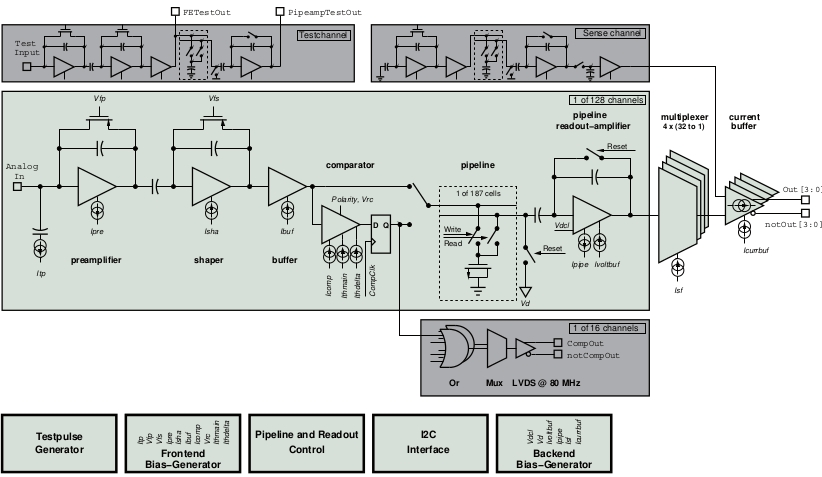
\includegraphics[scale=0.8]{rozdzial2/Beetle_block.jpeg}
 % Beetle_block.jpeg: 848x489 pixel, 96dpi, 22.44x12.94 cm, bb=0 0 636 367
 \caption{Schemat blokowy czipu Beetle\cite{Beetle}}
 \label{fig:Beetle_Block}
\end{figure}

Układ odczytuje 128 kanały VELO. Zbiór prądowych oraz napięciowych przedwzmacniaczy oraz kształtowników wykorzystywany jest do optymalizacji parametrów impulsu. 
Po ukształtowaniu impuls jest próbkowany a następnie w postaci analogowej przechowywany przez $4\mu s$ w linij opóźniającej (ang. pipeline) w oczekiwaniu na decyzję systemu wyzwalania pierwszego poziomu. Po akceptacji przez L0 dane przesyłane są do czterech kanałów analogowych. Każdy port wysyła dane z 32 fizycznych sensorów poprzedzone czterema pseudo-cyfrowymi nagłówkami.
Sygnały wyjściowe z układu Beetle przesyłane są przy pomocy 60 m kabli analogowych, w celu dalszej obróbki, do elektronicznych płyt akwizycyjnych TELL1 \cite{Aras}, co zostało zaprezentowane na rysunku \ref{sciezka}. Przy użyciu których sygnały są digitalizowane z 10 bitową precyzją a następnie przetwarzane przez układy FPGA (ang. Field Programmable Gate Arrays). 
\begin{figure}[ht]
 \centering
 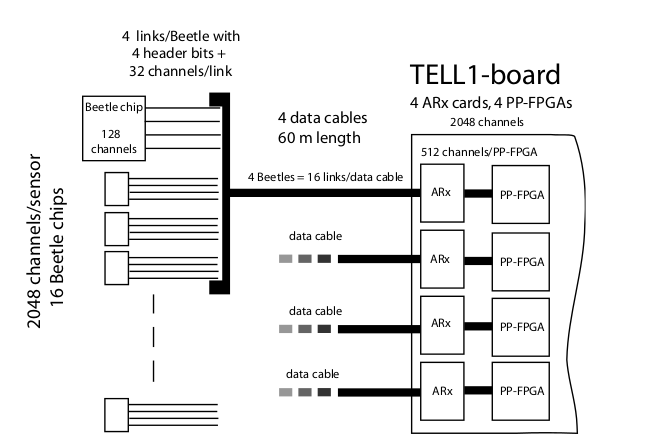
\includegraphics[scale=0.9]{rozdzial2/Velo_schematic.png}
 % Velo_schematic.png: 662x442 pixel, 96dpi, 17.51x11.69 cm, bb=0 0 496 331
 \caption{Ścieżka odczytowa pomiędzy kanałami VELO a płytą TELL1\cite{Aras}}
 \label{sciezka}
\end{figure}





\subsection{Detektory Czerenkowa}
RICH (ang. Ring Imaging Cherenkov detector) jest detektorem promieniowania Czerenkowa wykorzystywanym do identyfikacji hadronów. W szczególności wydajna i niezawodna separacja pionów oraz kaonów jest niezbędna przy badaniu rozpadów mezonów $B_{(s)}^0$ oraz $D_{(s)}^0$. W spektrometrze LHCb zamontowano dwa detektory RICH. Pierwszy z nich (RICH1), umieszczony zaraz za VELO, jest zoptymalizowany dla nisko pędowych cząstek o pędzie w przedziale $\sim 1- 60 GeV/c$. Drugi (RICH2), położony za magnesem, służy do identyfikacji cząstek o dużych pędach ($\sim 15-100 GeV/c$) \cite{RICH}. Detektor promieniowania Czerenkowa zbudowane są z radiatora, w którym cząstka emituje promieniowanie, oraz z układu luster skupiających odpowiednio promieniowanie na powierzchni fotoczułej. Pomiar kąta emisji promieniowania odbywa się przez pomiar promienia charakterystycznego pierścienia, który tworzy.
RICH1 znajduje się zaraz za detektorem wierzchołka, przed magnesem dipolowym. Radiatorem w nim jest aerogel (n = 1,03), który umożliwia identyfikacje kaonów dla przedziału pędów sięgających 2 GeV/c oraz odróżnienie pionów od kaonów, aż do 10 GeV/c  W RICH1 znajduje się drugi radiator:  $C_4F_{10}$(n=1,0015), który zapewnia rozróżnienie pion-kaon, w przedziale  50 GeV/c. Układem skupiającym jest lustro sferyczne o promieniu 1,7 m wykonane z
6 mm warstwy szkła pokrytej 900 nm warstwa glinu i 200 nm warstwa kwarcu. Do detekcji promieniowania użyto hybrydowych fotodetektorów umieszczone na powierzchnie sferycznej o promieniu dwa razy mniejszym niż zwierciadła.



\begin{figure}[th]
  \centering
  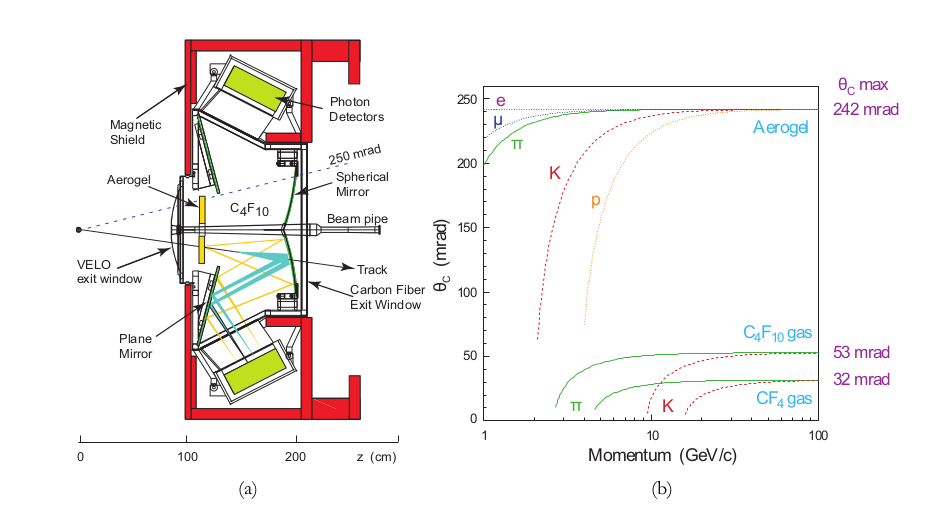
\includegraphics[scale=0.5]{rozdzial2/RICH.png}
  % TT-layout.jpg: 275x246 pixel, 100dpi, 6.99x6.25 cm, bb=0 0 198 177
  \caption{Schemat detektora RICH1	z zaznaczonymi ścieżkami dla światła pojawiającego się w aerożelu oraz $C_4F_{10}$(a). Rozkład kątów Czerenkowa w zależności od pędu cząstek emitujących. Rysunki pochodzą z  \cite{public}}
  \label{fig:RICH}
\end{figure}


\subsection{Detektory śladowe}
Układ detektorów śladowych pozwala na rekonstrukcję trajektorii cząstek oddziałujących z materiałem czynnym detektora. Składa się z części umieszczonych przed magnesem (VELO, TT) oraz za nim (stacje T1-T3 oraz komory mionowe). Umieszczony na rysunku \ref{fig:TTlayout} TT (ang. Tracker Turicensis) jest wykorzystywana w analizie do rekonstrukcji długożyciowych neutralnych cząstek np. kaonów rozpadających się na zewnątrz detektora VELO. Detektor ten zbudowany jest z czterech warstw krzemowych, mikropaskowych detektorów. 
\begin{figure}[th]
  \centering
  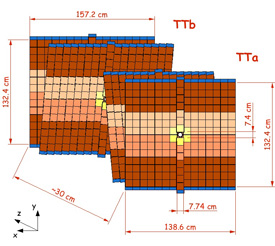
\includegraphics[scale=1]{rozdzial2/TT-layout.jpg}
  % TT-layout.jpg: 275x246 pixel, 100dpi, 6.99x6.25 cm, bb=0 0 198 177
  \caption{Schemat detektor TT \cite{public}}
  \label{fig:TTlayout}
\end{figure}
Detektory śladowe T1-T3,których schemat zamieszczono na rysunku \ref{fig:OTLayput},  dokonujące pomiarów pozycji za magnesem, dzielą się na dwie części. Pierwszą z nich jest IT (ang. Inner Tracker) zbudowany podobnie jak TT, z krzemowych mikropaskowych detektorów. Wynika to z faktu iż IT znajduje się w miejscu którym oczekiwane jest największa ilość cząstek, natomiast OT(ang. Outer Tracker) jest gazowym detektorem słomkowym.

\begin{figure}[th] 
  \centering
  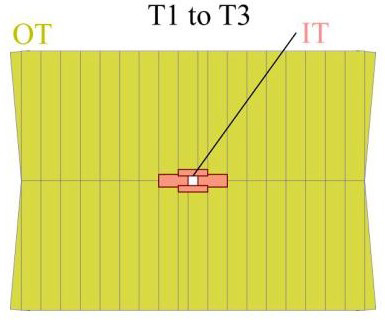
\includegraphics[scale=0.5]{rozdzial2/OT-Module-design.jpg}
  % OT-Module-design.jpg: 385x326 pixel, 100dpi, 9.78x8.28 cm, bb=0 0 277 235
  \caption{Schemat detektorów T1-T3\cite{public}. Region oznaczony na czerwono przedstawia IT natomiast na żółto zaznaczono OT.}
  \label{fig:OTLayput}
\end{figure}

\subsection{Kalorymetry}
Zadaniem  kalorymetrów jest identyfikacja fotonów, elektronów i hadronów oraz pomiar ich energii. Są wykorzystywane również w systemie wyzwalania. Wyróżniono następujące części:
\begin{itemize}
\item SPD (ang. Scintillator Pad Detector) oraz PS (ang. Pre Shower) służą do odróżniania fotonów i elektronów poprzez analizę topologii elektromagnetycznej kaskady cząstek wtórnych.
\item ECAL (ang. Electromagnetic CALorimeter) mierzy energię fotonów i elektronów. Zdjęcie detektora zostało zaprezentowane na rysunku \ref{fig:ECAl}.
\item HCAL (ang. Hadronic CALorimeter) używany do pomiaru energii hadronów.
\end{itemize}
\begin{figure}[th] 
  \centering
  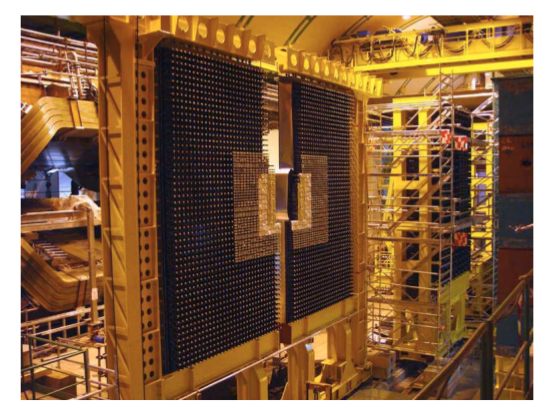
\includegraphics[scale=0.7]{rozdzial2/ECAL.png}
  % OT-Module-design.jpg: 385x326 pixel, 100dpi, 9.78x8.28 cm, bb=0 0 277 235
  \caption{Zdjęcie detektora ECAL po zamontowaniu go w detektorze LHCb.}
  \label{fig:ECAl}
\end{figure}



\subsection{Komory mionowe}
Identyfikacja mionów jest fundamentalnym wyzwaniem eksperymentu LHCb ponieważ cząstki te są stanami końcowymi powstającymi w wyniku rozpadów mezonów $B_{(s)}^0$ oraz $D_{(s)}^0$ . Miony, słabo oddziaływające z materią, są jedynymi cząstkami które przechodzą przez system kalorymetrów. Układ detektorów składa się z pięciu wielodrutowych komór proporcjonalnych. Mają bardzo ważną rolę w systemie wyzwalania L0, oraz estymacji pędu poprzecznego mionów. Struktura systemu detekcji mionów została zaprezentowana na rysunku \ref{fig:Muon}
\begin{figure}[H] 
  \centering
  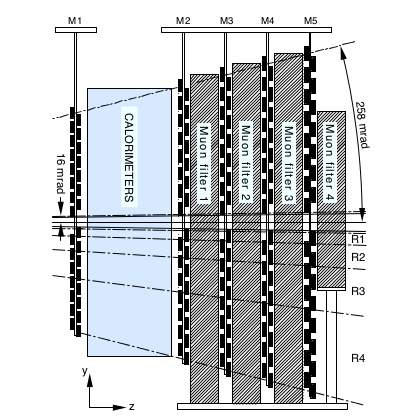
\includegraphics[scale=0.6]{rozdzial2/Muon.png}
  % OT-Module-design.jpg: 385x326 pixel, 100dpi, 9.78x8.28 cm, bb=0 0 277 235
  \caption{Schematyczne przedstawienie (widok z boku) stacji mionowych oraz żelaznych absorberów umieszczonych pomiędzy stacjami.}
  \label{fig:Muon}
\end{figure}


\subsection{System wyzwalania}
Częstotliwość oddziaływania wiązek protonowych wynosi 40MHz, co w przybliżeniu odpowiada strumieniowi danych 40TB/s. W celu jego ograniczenia zastosowano system wyzwalania (ang. trigger). Obecny system akwizycji jest w stanie archiwizować dane przychodzące z prędkością nie większą niż 200 MB/s(4kHz). Końcowy efekt uzyskany jest dzięki dwóm poziomom decyzyjnym.
\begin{itemize}
 \item Pierwszy poziom (Level0 [L0]) ogranicza  strumień danych z 40 MHz do 1.1MHz. Wykorzystuje on w procesie dokonywania decyzji fakt iż produkty rozpadów mezonów $B_{(s)}^0$ oraz $D_{(s)}^0$ posiadają stosunkowo wysoki pęd poprzeczny oraz energię. 
 \item Drugi poziom (High Level Trigger [HLT]) jest programem komputerowym wykonywanym na bardzo wielu CPU jednocześnie. Wykorzystuje dane pochodzące ze wszystkich detektorów. Szybki algorytm rekonstrukcji śladów łączy wyniki pochodzące z VELO wraz ze śladami zrekonstruowanymi przez pozostałe detektory śladowe. Na tej podstawie wybiera się przypadki fizyczne, które zapisywane są na dysku.  
\end{itemize}
\begin{figure}[ht]
  \centering
  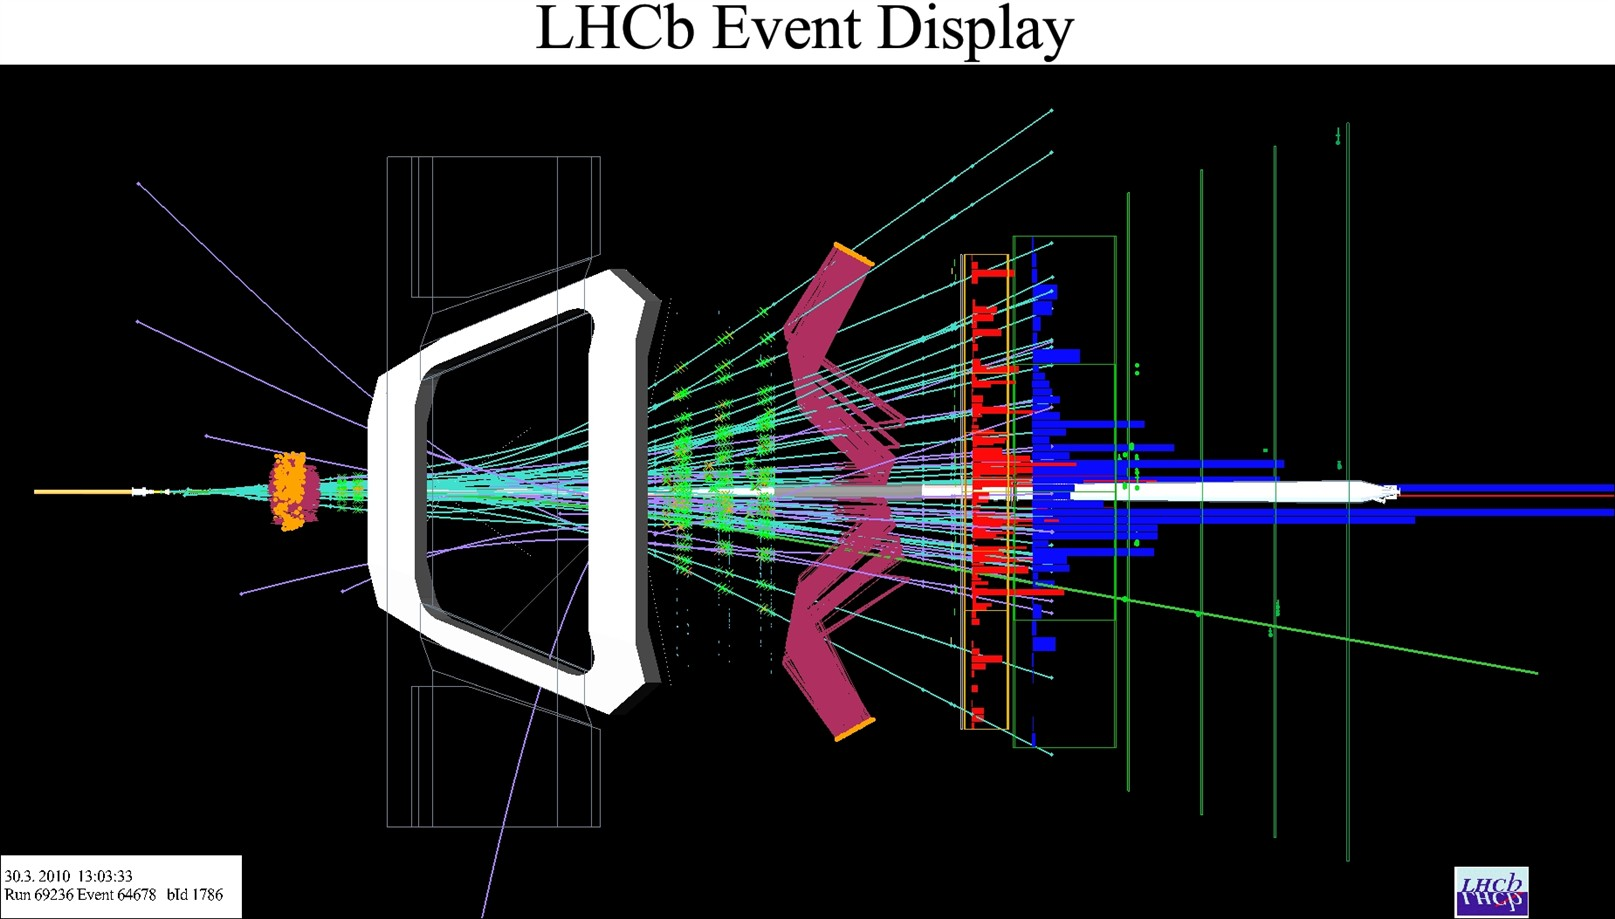
\includegraphics[scale=0.5]{rozdzial2/event.jpg}
  % event.jpg: 1615x919 pixel, 144dpi, 28.49x16.21 cm, bb=0 0 808 460
  \caption{Wizualizacja przypadku zdarzenia w detektorze LHCb\cite{event}}
  \label{fig:event}
\end{figure}
